\graphicspath{{images/mechanics}}

\section{Mechanik}

In der Nächsten Sektion wird die Mechanik der Fotobox beschrieben.
Die Mechanik ist ein sehr wichtiger Teil der Fotobox, da sie das erste
ist, was der Endbenutzer sieht. Sie sollte daher ansprechend und so stabil
aufgebaut sein, dass sie auch bei häufigem Transport nicht beschädigt wird.
Daher werde ich nun erläutern, warum ich mich für das aktuelle Design entschieden habe
und welche Probleme ich dabei hatte.

\subsection{Design}

Da das Design der Fotobox sehr wichtig ist, habe ich verschiedene Designs ausprobiert.
Der Weg, welcher zum schlussendlichen Design geführt hat, wird in Folgendem Unterkapitel beschrieben.

\begin{figure}[H]
    \centering
    
\includegraphics[width=1\textwidth]{fotobox_frontplatte_v1.png}
    \caption{Die erste Version der Frontplatte.}
    \label{fig:frontplatte_v1}
\end{figure}

In der \autoref{fig:frontplatte_v1} ist die erste Version der Frontplatte zu sehen.
Bei diesem Design, habe ich mich an schon am Markt erhältlichen Fotoboxen orientiert.
In den löchern eins und zwei sollten jeweils ein Blitz und eine LED Lampe platziert werden,
in dem mittleren Loch mit der Nummer drei sollte die Kamera platziert werden.


Jedoch hat sich herausgestellt, dass diese Design, durch die seitliche Platzierung des Blitzes
das Bild nicht einheitlich ausleuchtet, und einen seitlichen Schatten hinter dem 
Motiv wirft. Was die Qualität der Bilder, wie in \autoref{fig:seitlicher_blitzt}
zu sehen ist, deutlich verringert, da das Bild auch nicht einheitlich ausgeleuchtet wird.

\newpage
\begin{figure}[H]
    \centering
    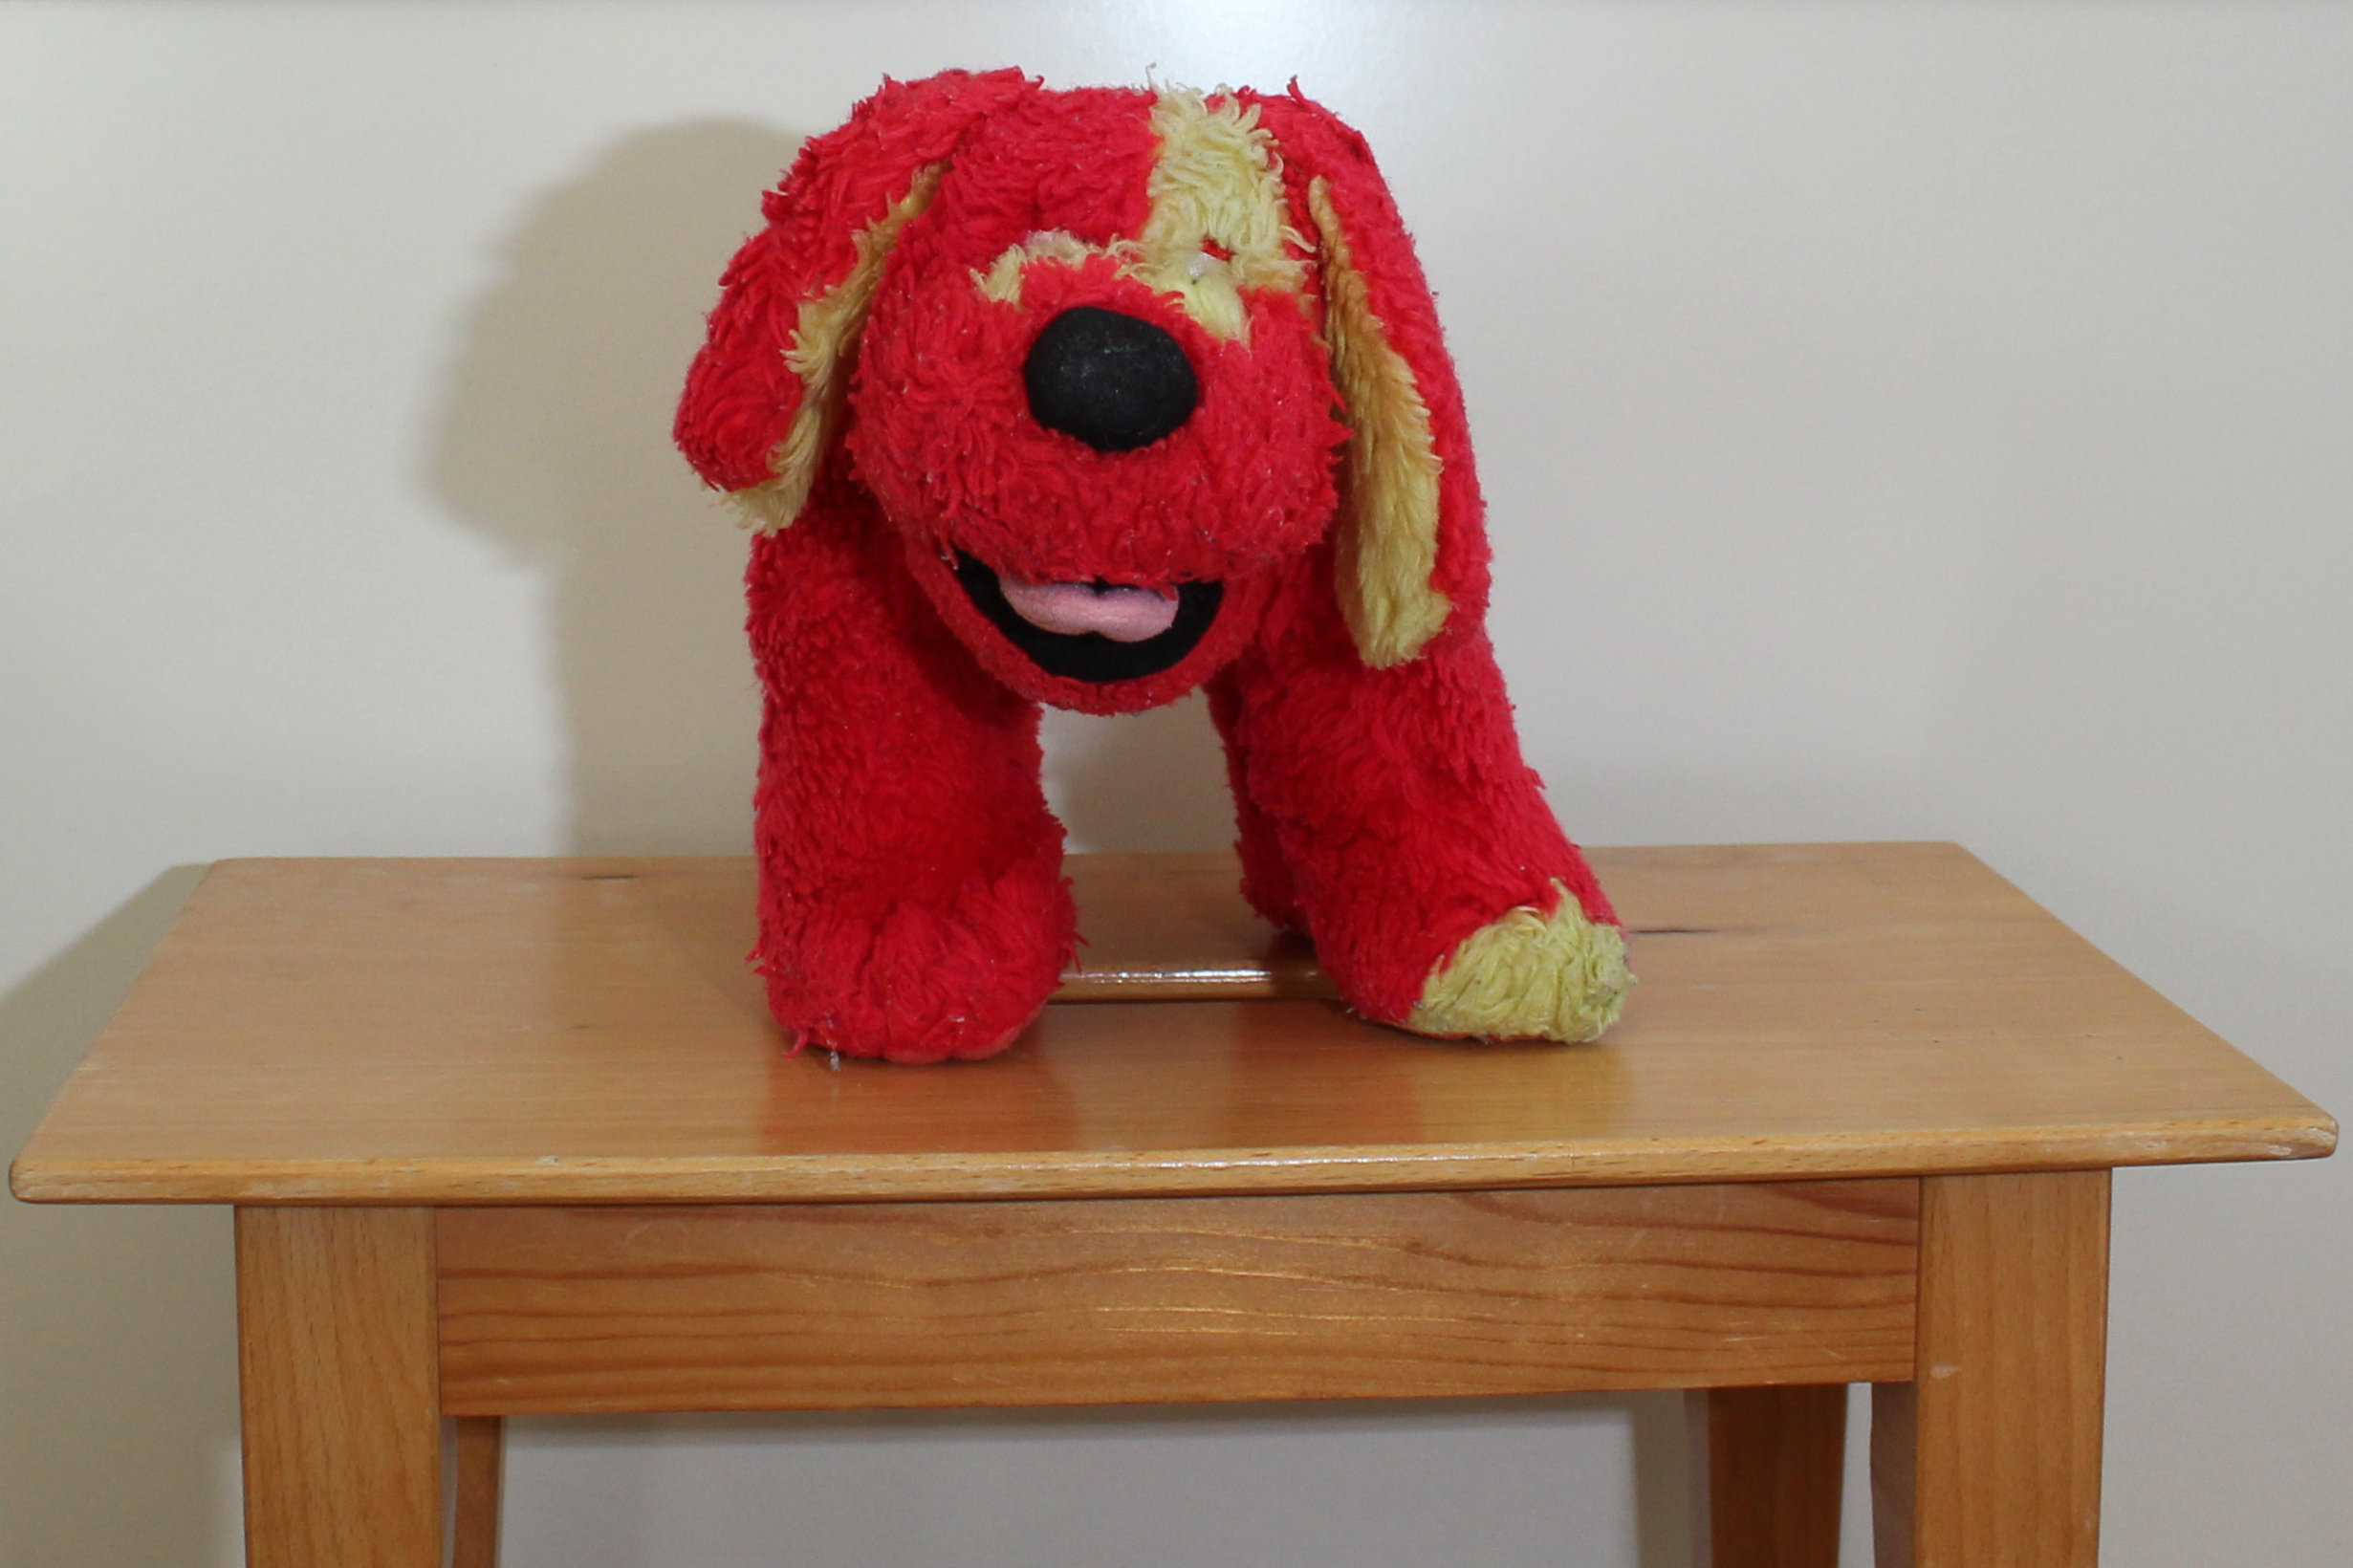
\includegraphics[width=0.8\textwidth]{blitz_seitlich.JPG}
    \caption{Beispielbild mit seitlichem Blitz.}
    \label{fig:seitlicher_blitzt}
\end{figure}

In der \autoref{fig:seitlicher_blitzt} ist zu sehen, dass durch die seitliche Platzierung des Blitzes 
auf der linken Seite neben dem Motiv ein Schatten entsteht. Dieser Schatten ist unerwünscht und sollte
durch ein zentrales Blitzlicht vermieden werden.

\begin{figure}[H]
    \centering
    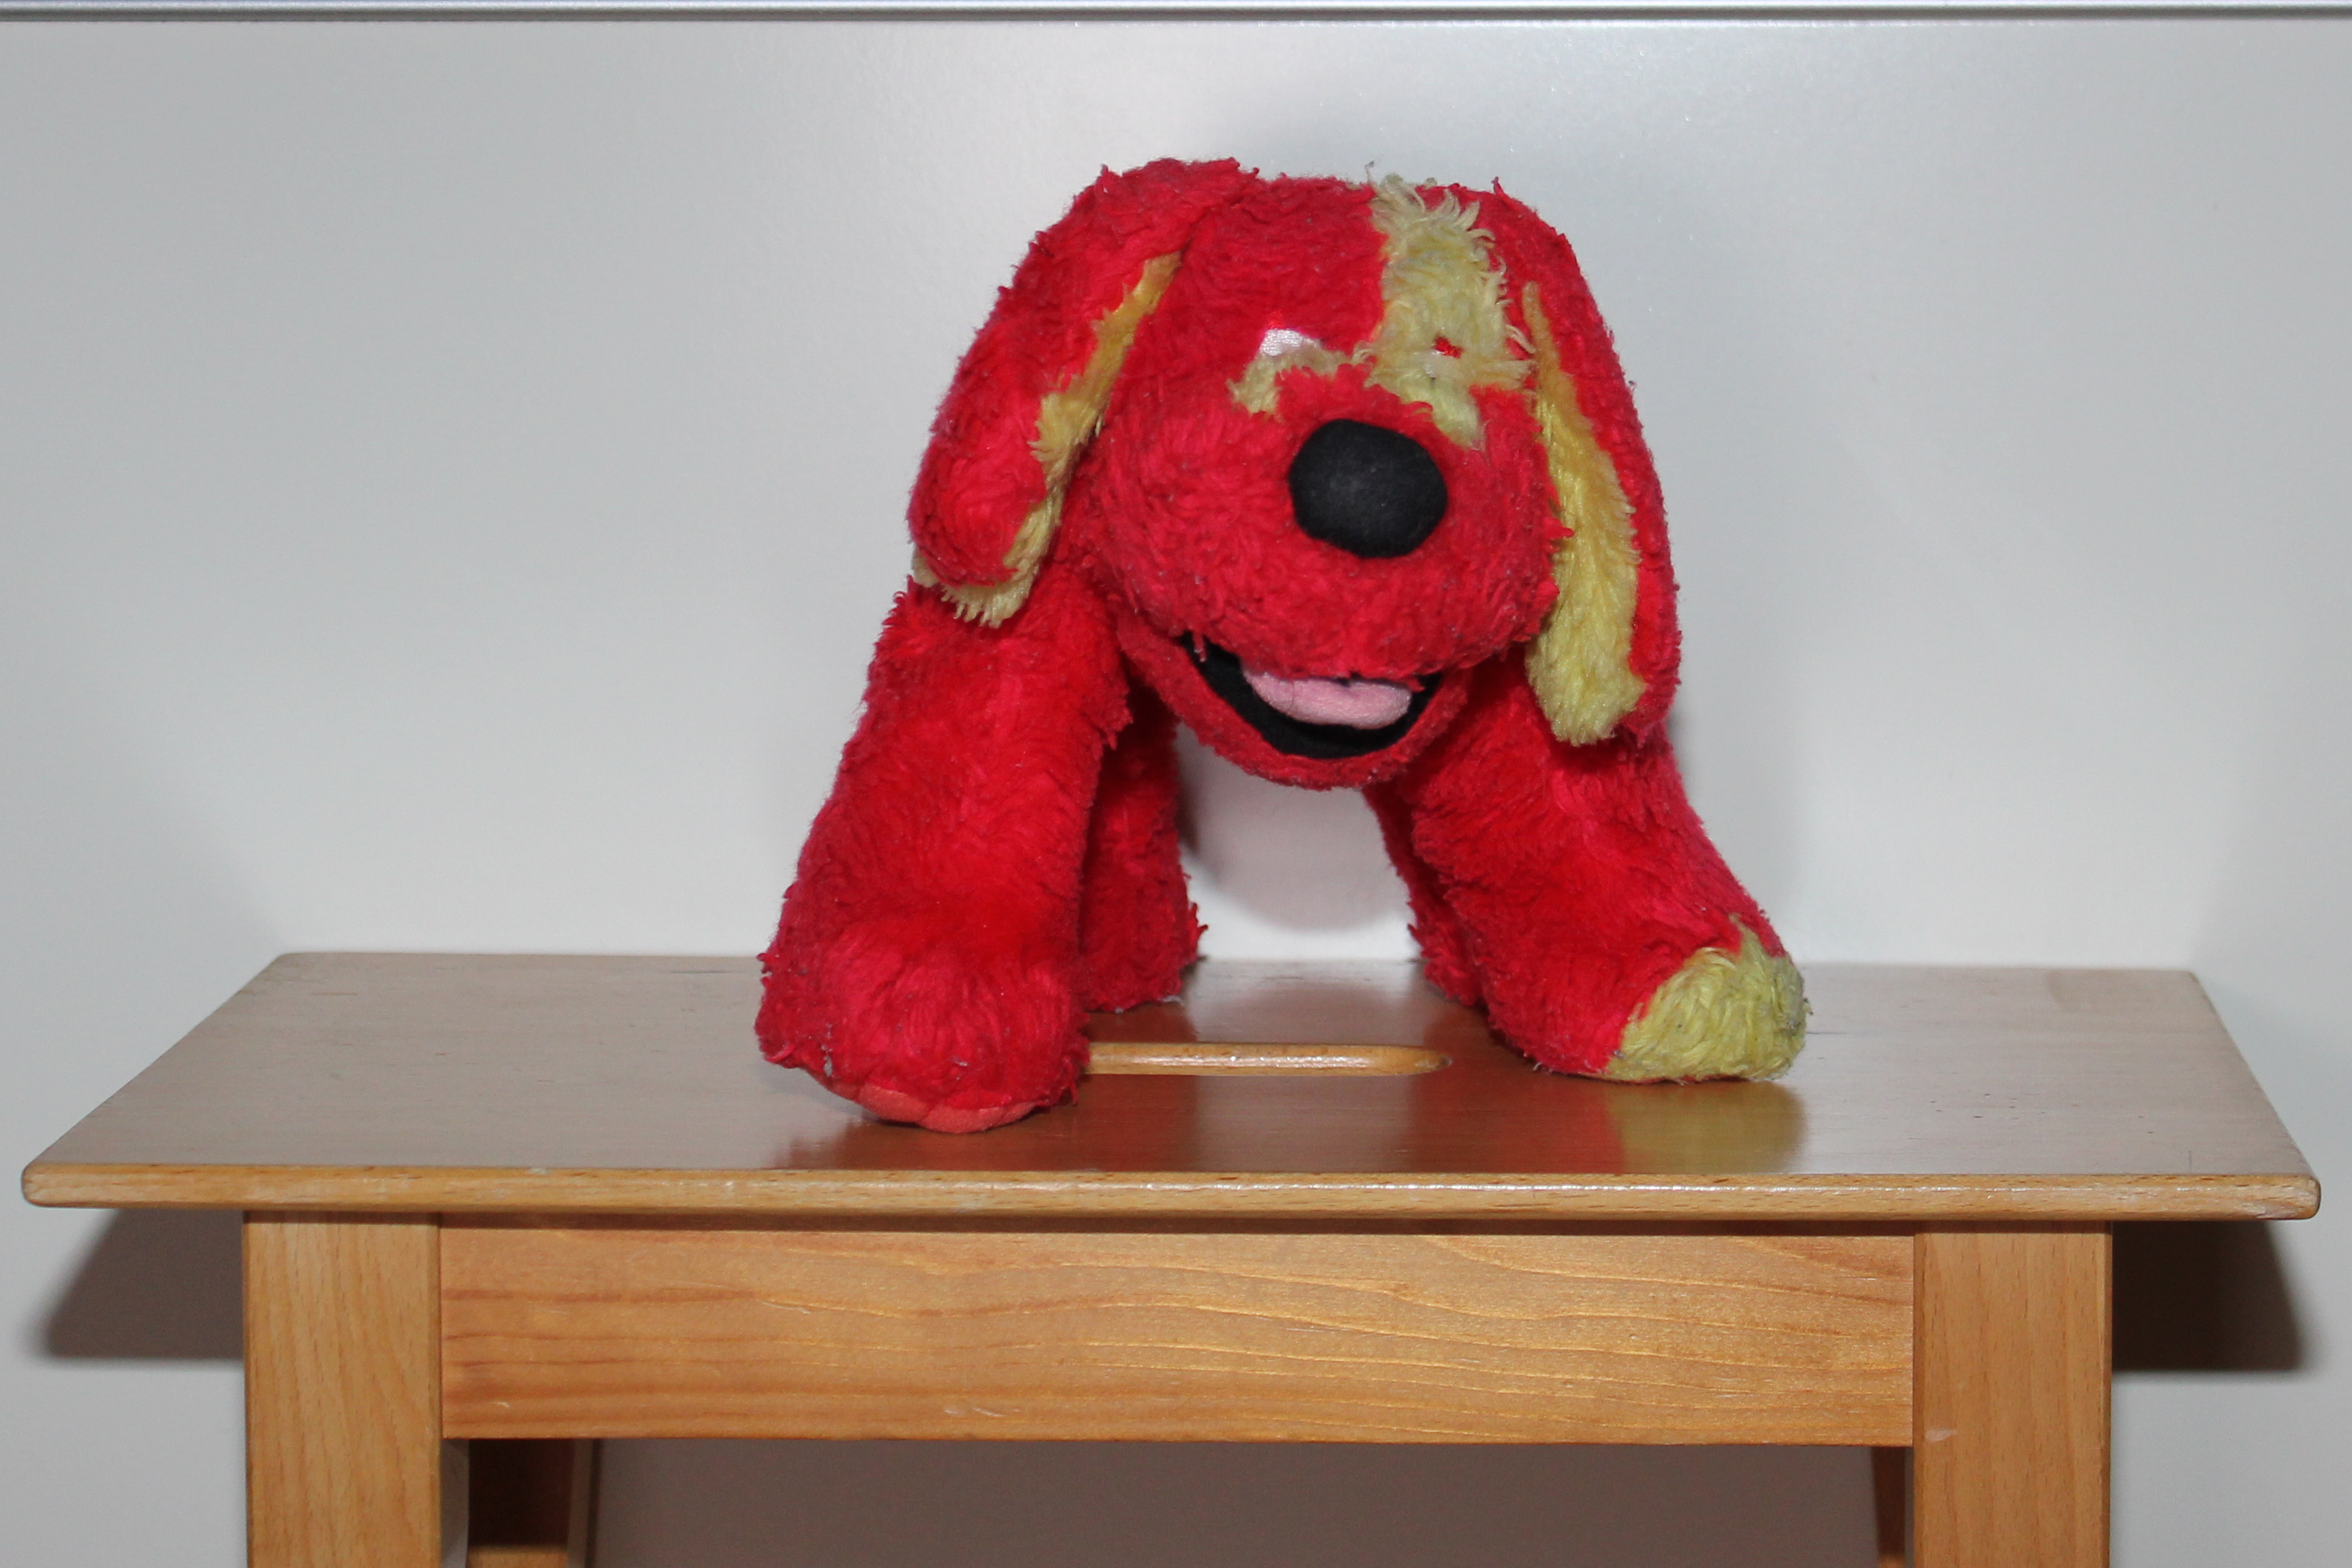
\includegraphics[width=0.8\textwidth]{blitz_vorne.JPG}
    \caption{Beispielbild mit zentralem Blitz.}
    \label{fig:zentraler_blitz}
\end{figure}

In der \autoref{fig:zentraler_blitz} ist zu sehen, dass durch die zentrale Platzierung des Blitzes,
das Bild deutlich besser ausgeleuchtet ist und keine seitlichen Schatten entstehen. 

\newpage

Um dieses Problem zu lösen, habe ich die Frontplatte umdesignt. 
Wie in \autoref{fig:frontplatte_v2} zu sehen ist, ist das neue Design 
nun höher, wie breit, wodurch es möglich ist, den Blitzt oberhalb der Kamera in 
Öffnung eins zu platzieren. In den Öffnungen zwei und drei sind die LED Lampen,
durch die auch bei der Vorschau eine gute Ausleuchtung erzielt wird.

\begin{figure}[H]
    \centering
    
\includegraphics[width=0.75\textwidth]{fotobox_frontplatte_v2.png}
    \caption{Die erste Version der Frontplatte.}
    \label{fig:frontplatte_v2}
\end{figure}

Dieses Design hat auch noch andere Vorteile, wie zum Beispiel, dass es einem Gesicht 
ähnelt, was den psychologischen Effekt hat, dass sich die Menschen wohler fühlen,
da sie das Gefühl haben, dass sie jemanden ansehen und nicht nur eine Holzbox.

\newpage

\subsection{Zusammenbau}

Im folgenden Kapitel wird der Zusammenbau der Fotobox beschrieben.
Da die Fotobox aus mehreren Teilen besteht, welche alle zuerst Zugeschnitten,
und alle nötigen Öffnungen gebohrt und gefräst werden müssen.

\subsubsection{Rohmaterial}

Das Rohmaterial, für welches ich mich entschieden habe, ist 18 mm dickes buchen
Leimholz, wie in \autoref{fig:rohmaterial} zu sehen ist.

\begin{figure}[H]
    \centering
    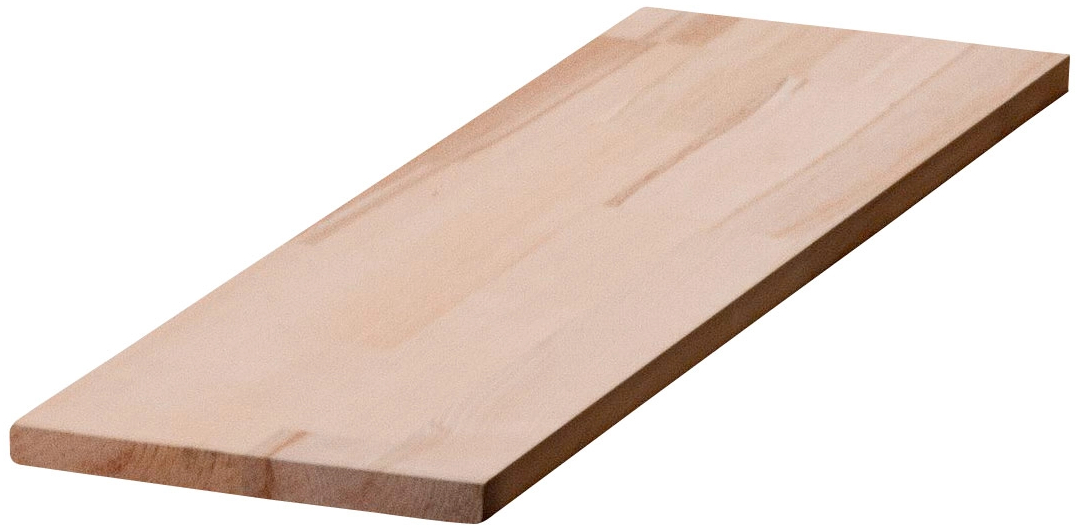
\includegraphics[width=0.75\textwidth]{rohmaterial.JPG}
    \caption{Das Rohmaterial der Fotobox.}
    \label{fig:rohmaterial}
\end{figure}

Ich habe mich für Leimholz aus Buche entschieden, da es durch die Verleimung der
einzelnen Holzlamellen eine hohe Formstabilität aufweist und sich kaum verzieht.
Zudem ist Buche ein sehr hartes Holz, wodurch die Box sehr stabil ist.
Jedoch ist Buche durch diese Eigenschaften auch schwerer zu verarbeiten,
als ein weicheres Holt und durch das höhere Gewicht, wird die Box auch schwerer.

\newpage

\subsubsection{Zuschnitt}